

\section{Experiment}
\label{si:experiment}

\section{Jump Sizes $\Delta r$}

Euclidean distance : 

\begin{equation}
\Delta r = d(p, q) = \sqrt{(p_1- q_1)^2 + (p_2 - q_2)^2+\cdots+(p_i - q_i)^2+\cdots+(p_n - q_n)^2}.
\end{equation}

with $n=8$ (3-nodes BayesNet) or $n=16$ (4-npdes BayesNet) and $p$,$q$, 2 consecutive position vectors

\begin{figure}[h!]
\begin{center}
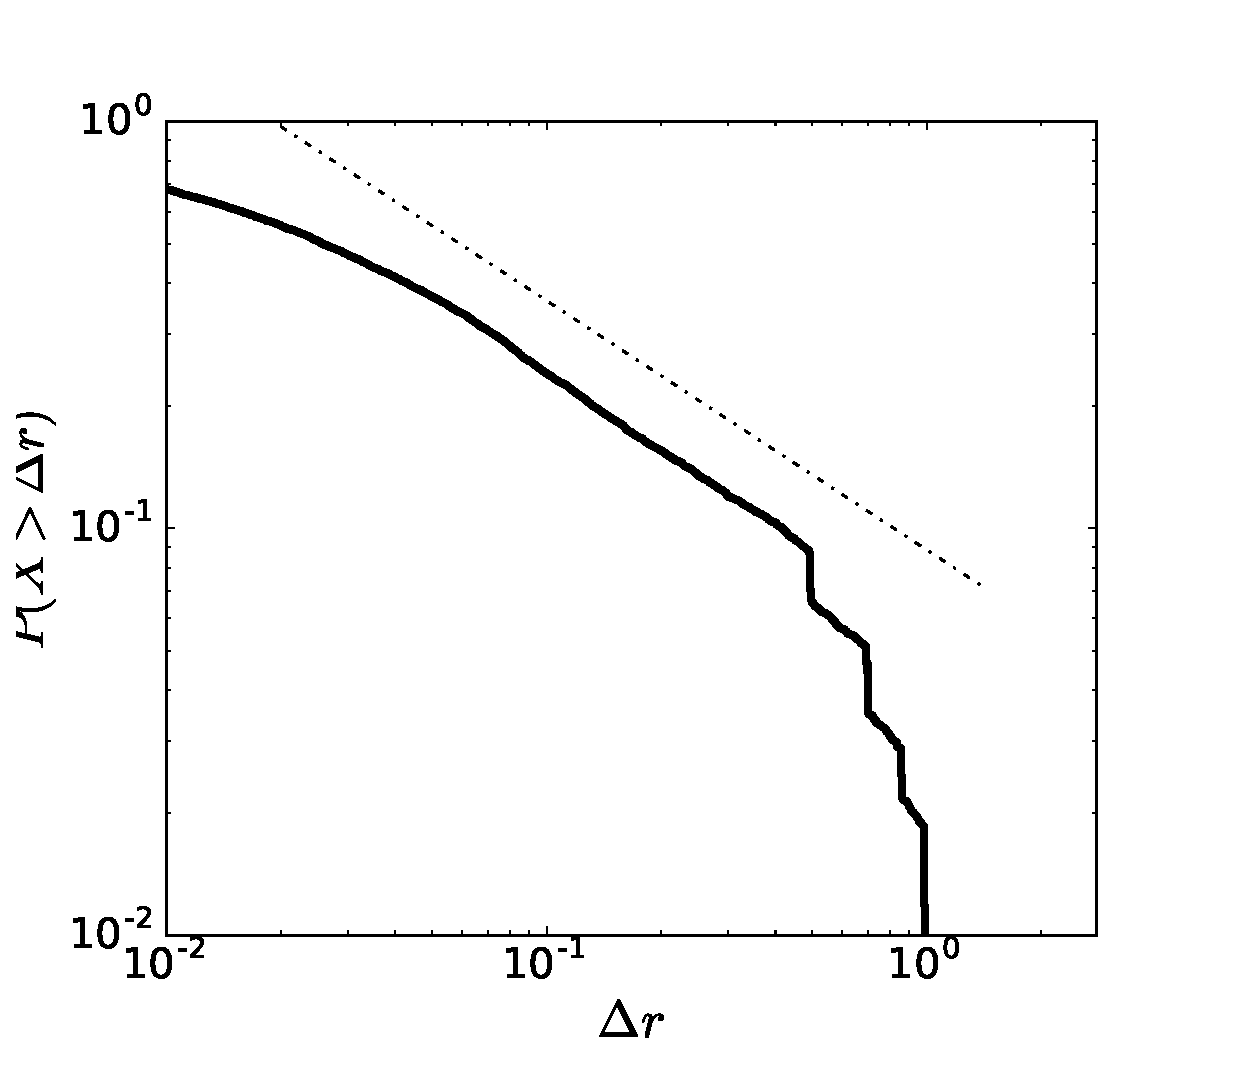
\includegraphics[width=10cm]{figures/CCDF_Displacement_simple.eps}
\caption{(3-node BayesNet) : exponent $\alpha = 0.61(3)$ with upper cutoff  $x_{max} \approx 1.4$ (theoretical limit is $x_{max} = 2\sqrt{2}$).}
\label{fig:jump_sizes}
\end{center}
\end{figure}


\section{Waiting Times $\Delta t$}



\begin{figure}[h!]
\begin{center}
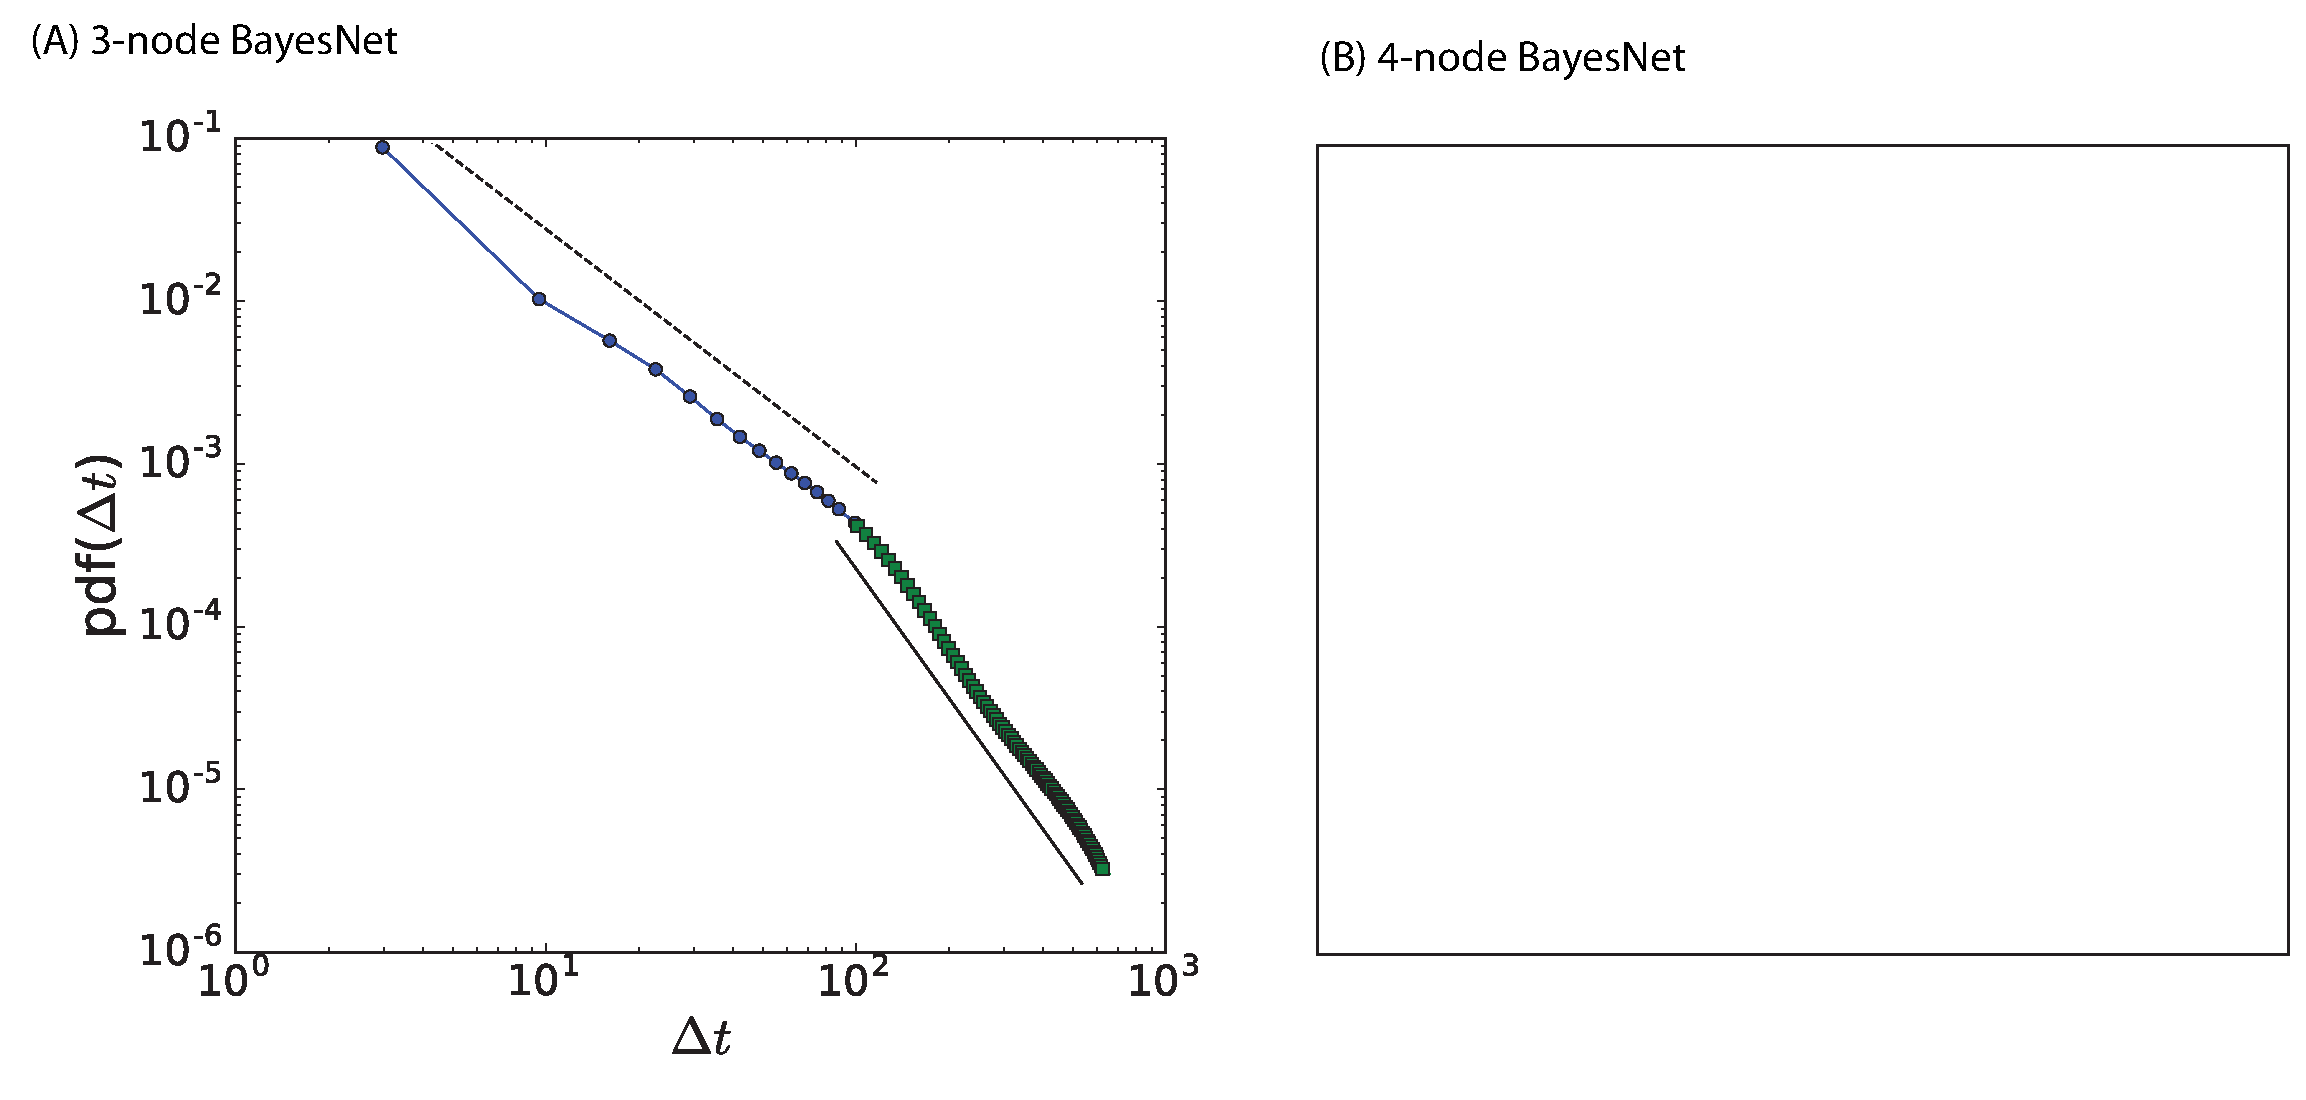
\includegraphics[width=15cm]{figures/dt_kernel_SI.eps}
\caption{Distribution of Waiting Times (fitted by kernel density estimators \cite{}) exhibits a change of regime typical of changes of regimes in waiting times \cite{maillart2011,saichevTheory}: $\beta_{\Delta t  \leqslant 100} \approx 0.46(3)$ (slope $\sim t^{-(1+ \beta_{\Delta t  \leqslant 100})}$ represented by dashed line) and $\beta_{\Delta t > 100} \approx 1.65(1)$ (slope $\sim t^{-(1+ \beta_{\Delta t  > 100})}$ represented by continuous line).}
\label{fig:waiting_times}
\end{center}
\end{figure}


\section{Correlation $\Delta r$ and $\Delta t$}
\label{si:corr_dr_dt}


\begin{figure}[h!]
\begin{center}
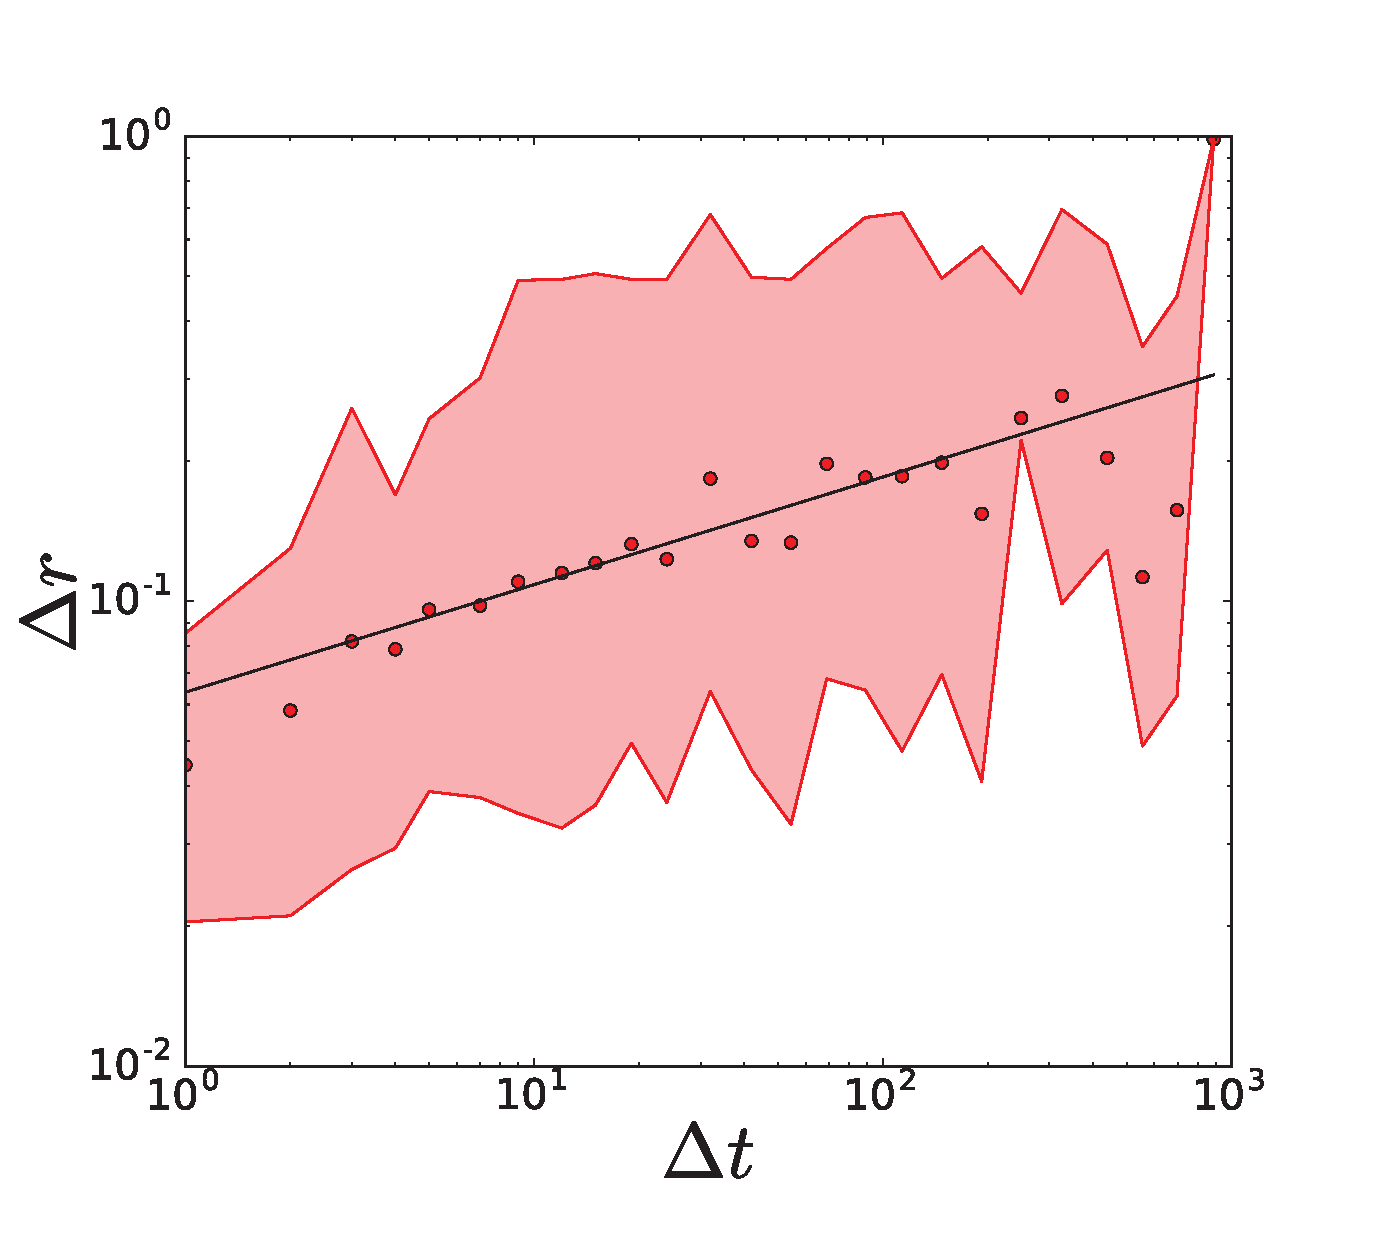
\includegraphics[width=10cm]{figures/cor_Delta_t_Delta_r_simple.eps}
\caption{3-node BayesNet : Correlation (Spearman rank correlation) between $corr(\Delta r,\Delta t) \approx 0.32$, and the main direction of dependence can be approximated by a scaling function $\Delta r \sim {(\Delta t)}^{0.23(2)}$ (least square fit of values in double logarithmique scale, $p < 0.001$ and $R= 0.21$}
\label{fig:corr_dr_dt}
\end{center}
\end{figure}




